\section{Differentialgleichungen}
\subsection{Differentialgleichungen}
\begin{definition}{Definition Differentialgleichung}\\
  \begin{itemize}
    \item Eine Differentialgleichung \(n\)-ter Ordnung ist ein Gleichung von der Form:
      \[F(x,y,y',y'',\ldots,y^{(n)})=0\]
      für eine gesuchet Funktion \(y=y(x)\), in der Ableitungen von \(y(x)\) bis zur \(n\)-ten Ordnung auftreten.
    \item Falls die DGL nach \(y^{(n)}\) aufgelöst ist, nennt man sie explizit, ansonsten implizit.
      Oft können implizite DGL durch einfaches Umformen in explizite DGL umgewandelt werden.
  \end{itemize}
\end{definition}
\begin{definition}{Arten von DGL}\\
  \begin{itemize}
    \item Eine DGL heisst seperierbar, falls \(F(x,y)\) als Produkt eines \(x\)- und eines \(y\)-Anteils geschrieben
      werden kann, d.h. es hat die Form:
      \[y'=g(x)\cdot h(y)\]
      für irgendwelche Funktionen \(g(x)\) und \(h(y)\)
    \item Eine DGL heisst autonom, falls \(F(x,y)\) nur von \(y\) abhängt, d.h. es hat die Form:
      \[y'=f(y)\]
    \item Eine DGL heisst linear, falls die Variabel welche abgeleitet wird nur in der ersten Potenz vorkommt und nicht
      multipliziert miteinander oder mit der unabhängigen Variabel wird.
  \end{itemize}
\end{definition}
\begin{definition}{Definition Anfangswertproblem}\\
  \begin{itemize}
    \item Eine DGL mit Anfangsbedingun ist ein Anfangswertproblem.
    \item Ein Anfangswertproblem \(n\)-ter Ordnung ist:
      \[\left\{\begin{tabular}{rcl}
	  \( F(x,y,y',y'',\ldots,y^{(n)})\)&\(=\)&\(0,\;(x,y,\ldots,y^{(n)})\in \Omega\)\\
	  \(y(x_0)\)&\(=\)&\(y_0\)\\
	  \(y'(x_0)\)&\(=\)&\(y_1\)\\
		\(\) &\(\vdots\)&\(\)\\
	 \( y^{n-1}(x_0)\)&\(=\)&\( y_{n-1}\)
      \end{tabular}\right.\]
    \item Anfangswertproblem für explizite DGL 1. Ordnung:
      \[\left\{\begin{tabular}{rcl}
	  \(y'\)&\(=\)&\(G(x,y),\quad (x,y,y')\in \Omega\subseteq\mathbb{R}\times\mathbb{R}^2\)\\
	  \(y(x_0)\)&\(=\)&\(y_0\)
      \end{tabular}\right.\]
    \item Die Menge aller Lösungen einer DGL nennt man die allgemeine Lösung der DGL.
    \item Die Lösung einse Anfangswertproblems nennt man eine spezielle bzw. partikuläre Lösung der DGL.
  \end{itemize}
\end{definition}
\subsection{Richtungsfeder}
\begin{definition}{Definition Richtungsfeld}\\
  \begin{itemize}
    \item Ein Richtungsfeld ist ein geometrisches Verständnis von expliziten DGL 1. Ordnung, d.h. DGL der Form:
      \[y'=f(x,y)\]
    \item \(f(x,y)\) gibt also die Steigung der Lösungskurve am Punkt \((x,y)\) an:
  \begin{center}
  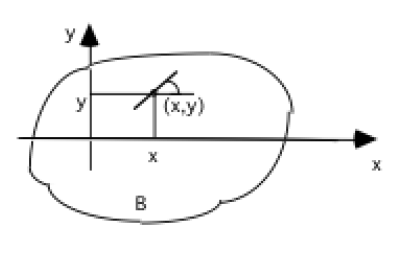
\includegraphics[width=0.4\textwidth]{images/Richtungsfeld.png}
  \end{center}
    \item Jeder Punkt ist somit die Tangente einer spezifischen Lösungskurve
  \begin{center}
  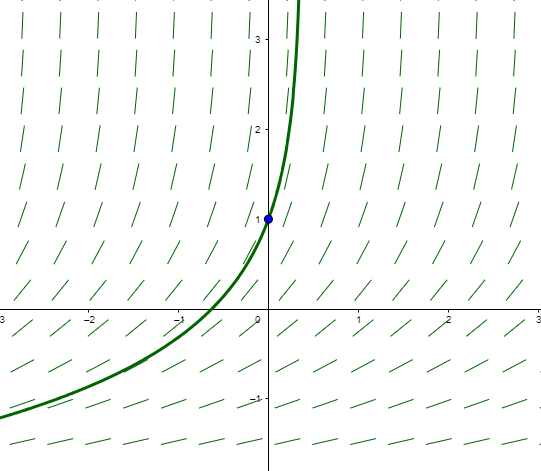
\includegraphics[width=0.4\textwidth]{images/RichtungsfeldKurve.png}
  \end{center}
  \end{itemize}
\end{definition}
\begin{definition}{Richtungsfelder von Speziellen DGL}\\
  \begin{itemize}
    \item Unbestimmtes Integral: \(y'=f(x)\), das Richtungsfeld ist unabhängig von \(y\) die verschiedenen Lösungen
      unterscheiden sich nur durch eine verschiebung in \(y\)-Richtung durch die Konstante \(C\).
  \begin{center}
  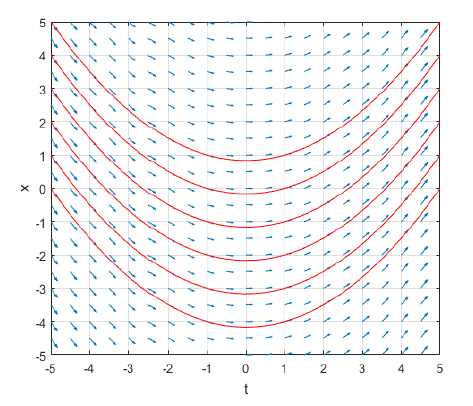
\includegraphics[width=0.4\textwidth]{images/UnbestimmtesIntegral.png}
  \end{center}
\item Autonome DGL:\(y'=f(y)\), das Richtungsfeld ist unabhängig von \(x\) die Verschiedenen Lösungen gehen durch
  Verschiebung in \(x\)-Richtung in einander über.
  \begin{center}
  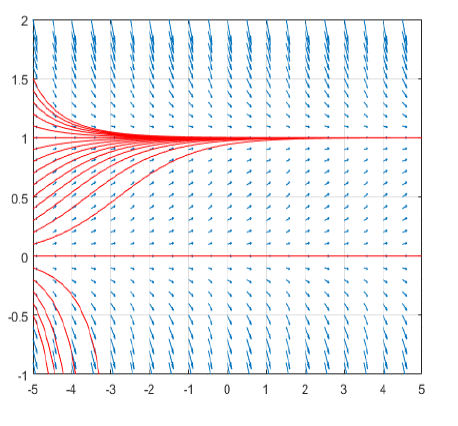
\includegraphics[width=0.4\textwidth]{images/AutonomeDGL.png}
  \end{center}
  \end{itemize}
\end{definition}
\begin{KR}{Lösen von Seperierbaren Differentialgleichungen}\\
  \begin{itemize}
    \item DGL:
      \[\frac{\mathrm{d}y}{\mathrm{d}x}=g(x)\cdot h(y)\]
    \item Falls \(h(y_0)=0\), ist \(y=y_0\) eine Lösung der DGL.
    \item Trennung aller \(x\)- und \(y\)-Terme:
      \[\frac{1}{h(y)}\cdot \mathrm{d}y=g(x)\cdot \mathrm{d}x\]
    \item Integration auf beiden Seiten:
      \[\int{\frac{1}{h(y)}\mathrm{d}y}=\int{g(x)\mathrm{d}x}\]
    \item Auflösen nach \(y\), Anfangsbedingungen einsetzen:
      \[\int_{y_0}^{y}{\frac{1}{h(s)}\mathrm{d}s}=\int_{x_0}^{x}{g(t)\mathrm{d}t}\]
  \end{itemize}
\end{KR}
\begin{formula}{Formel für inhomogene Differentialgleichungen}
  \begin{itemize}
    \item Die allgemeine Lösung der inhomogenen Differentialgleichung:
      \[y'+f(x)y=g(x)\]
      ist gegeben durch:
      \[y=e^{-F(x)}\cdot \int{g(x)e^{F(x)}\mathrm{d}x}\]
      wobei \(F(x)\) eine Stammfunktion von \(f(x)\) ist.
  \end{itemize}
\end{formula}
\begin{definition}{Lösung von Anfangswertproblemen mit seperiarbaren DGL}
  \begin{itemize}
    \item Sind \(g(x)\) und \(h(y)\) stetige Funktionen und \((x_0,y_0)\in \mathbb{R}^2\) mit \(h(y_0)\neq 0\), hat das
      Anfangswertproblem:
      \[\left\{\begin{tabular}{rcl}
	  \(y'\)&\(=\)&\(g(x)h(y)\)\\
	  \(y(x_0)\)&\(=\)&\(y_0\)\\
      \end{tabular}\right.\]
      genau eine Lösung. Sie kann gefunden werden, indem beide Seiten von 
      \[\int_{y_0}^{y}{\frac{1}{h(s)}\mathrm{d}s}=\int_{x_0}^{x}{g(t)\mathrm{d}t}\]
      berechnet werden und nach \(y\) aufgelöst werden.
  \end{itemize}
\end{definition}
\subsection{Numerische Verfahren}
\begin{definition}{Eulerverfahren}
  \begin{itemize}
    \item Gleichung einer beliebigen Geraden mit Steigung \(m\) am Punkt \((x_k,y_k)\):
      \[y=y_k+m\cdot(x-x_k)\] 
      Graphisch:
  \begin{center}
  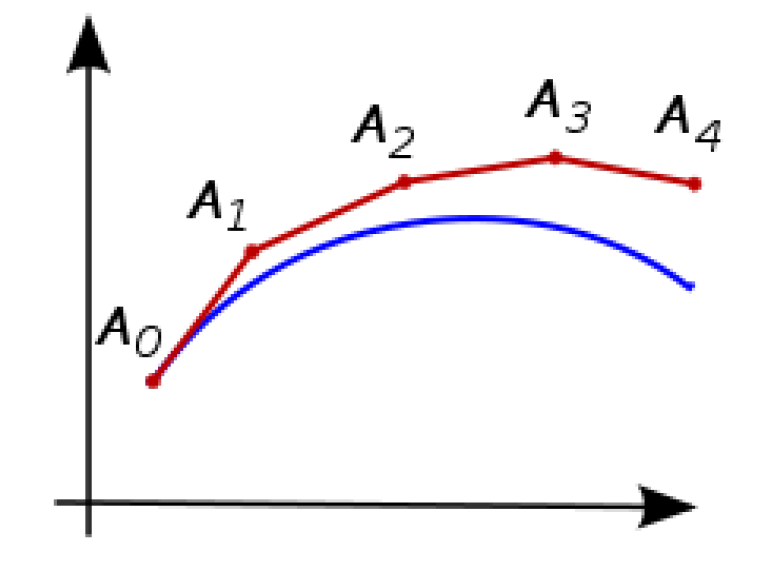
\includegraphics[width=0.4\textwidth]{images/Newtonverfahren.png}
  \end{center}
      DGL am Punkt \((x_k,y_k)\):
      \[y=y_k+f(x_k,y_k)\cdot (x-x_k)\]
    \item Für \(k=0 \text{ und } x=x_0\):
      \[\underbrace{y_1}_{\approx y(x_1)}=y_0+f(x_0,y_0)\cdot\underbrace{(x_1-x_0)}_{=h}\]
    \item Algorythmus für beliebige \(k\):
      \[\left\{\begin{tabular}{rcl}
	  \(x_k\)&\(=\)&\(x_0+k\cdot h\)\\
	  \(y_{k+1}\)&\(=\)&\(y_k+h\cdot f(x_k,y_k)\)
	\end{tabular}
      \right.\]
    \item Problem: Die steigung wird nur am linken Ende des Intervalls berücksichtigt!
    \item Lösung: Verbesserte numerische Verfahren!
  \end{itemize}
\end{definition}
